\newpage
\section{More Playing with Blocks}\label{A:B2}\index{base-ten blocks} 
%Did you put your blocks away? Darn---there is still more to be
%done! Just so that we are all on the same page, here are the basic
%blocks:
%\[
%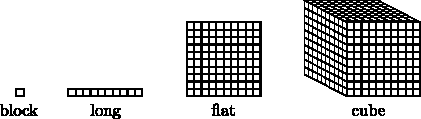
\includegraphics{../graphics/baseTenBlocks.pdf}
%\]

\begin{prob}
Now Oscar is modeling the basic multiplication algorithm:
\[
\begin{tabular}{@{}r@{}}
11~~\\
234\\
$\times$~~3\\ \hline
702
\end{tabular}
\]
\[
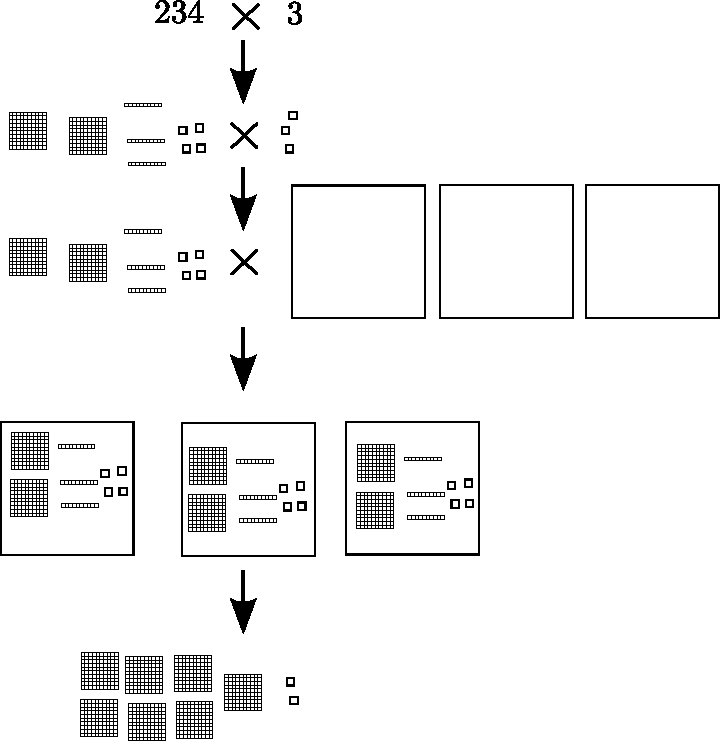
\includegraphics[scale=0.9]{../graphics/oscarMult.pdf}
\]
Can you explain what is going on?  Does his model illustrate the algorithm?  If so, explain how.  If not, describe how to use base ten blocks to explain the algorithm.  
\end{prob}

\begin{teachingnote}
This model doesn't show the separate steps in the algorithm.  It creates the three copies of 243 all at once rather than one place value at a time.  

The standard algorithm can be explained with blocks:  
\begin{itemize}
\item Three copies of four blocks makes 12 blocks.  Regroup as 1 long and 2 blocks. Write 2 below in blocks column and 1 above in longs column.
\item Three copies of three longs makes 9 longs.  Plus 1 long (from regrouping) makes 10 longs.  Regroup as 1 flat and 0 longs.  Write 0 below in the longs column and 1 above in the flats column.  
\item Three copies of 2 flats makes 6 flats.  Plus 1 flat (from regrouping) makes 7 flats.  Write 7 below in the flats column.  
\end{itemize}

And here is the ``behind the scenes algebra.''

\begin{align*}
234 \times 3 & = (2\cdot 10^2 + 3\cdot 10 + 4)\times 3 \\
&= 3\cdot 2\cdot 10^2 + 3\cdot 3\cdot 10 + 3\cdot 4 \\
&= 3\cdot 2\cdot 10^2 + 3\cdot 3\cdot 10 + 12 \\
&= 3\cdot 2\cdot 10^2 + 3\cdot 3\cdot 10 + 10 + 2\\
&= 3\cdot 2\cdot 10^2 + (3\cdot 3 + 1)\cdot 10 + 2\\
&= 3\cdot 2\cdot 10^2 + 10 \cdot 10 + 2\\
&= (3\cdot 2 + 1) \cdot 10^2 + 0 \cdot 10 + 2\\
&= 7\cdot 10^2 + 0 \cdot 10 + 2\\
&=702
\end{align*}
\end{teachingnote}

 
\begin{prob}
Here is an example of the basic division algorithm:
\[
3\,\begin{tabular}[b]{@{}r@{}r} 
67 &\, R$1$\\ 
\cline{1-1}
\Big)\begin{tabular}[t]{@{}l@{}} 202\\ 
18 \\ 
\divrule{0}{2}  ~22 \\
 ~21\\
 \divrule{1}{2}
~~1
\end{tabular}
\end{tabular}
\]
Explain how to model this algorithm with base-ten blocks, assuming that you start with 202 as two flats and two blocks and that you intend to organize them into three equal piles.  
\end{prob}

\begin{teachingnote}
\begin{itemize}
\item Encourage both 3 groups and groups of 3.  
\item For $202\div 3$, 3 doesn't go into 2 flats.  Regroup the 2 flats as 20 longs.  Then 3 groups gives 6 longs with for a total of 18 longs.  After subtraction, 2 longs are remaining. 
\item Regroup the 2 remaining longs as 20 blocks and combine with the 2 blocks to give 22 blocks.  
\item Organize the blocks into 3 groups give 7 blocks in each group for a total of 21 blocks.  After subtraction 1 block remains.  
\end{itemize}
\end{teachingnote}
